%
% Copyright (c) 2011-2013, fortiss GmbH.
% Licensed under the Apache License, Version 2.0.
% 
% Use, modification and distribution are subject to the terms specified
% in the accompanying license file LICENSE.txt located at the root directory
% of this software distribution. A copy is available at
% http://chromosome.fortiss.org/.
%
% This file is part of CHROMOSOME.
%
% $Id$
%

% =================================================================
\section{Example 7: Configurator Extension (15 minutes)}
\label{sec:example_configuratorExtension}
% =================================================================

This examples shows the \textit{configurator extension} concept,
together with \textit{lower} and \textit{upper connection bounds} for input ports.
It is located in the directory \texttt{examples/configuratorExtension/}. 

The \textit{configurator extension} component of \xme allows to register configurators
that react on changes in the system configuration. Currently you can only
register configurators for the logical route graph.
After each change in the graph, for example after a plug~\&~play event, all
registered configurators will be called.
In the configurator you can inspect the current routes.
You can also add and remove\footnote{Not supported yet.} components, as
well as removing routes\footnote{Only supported for non-established routes.}.

\textit{Connection bounds} specify restrictions on the number of routes that an input
port is allowed to be connected to.
This is specified in the manifest of the component.
Currently this information is available at runtime~--~for example in a configurator~--~
but not enforced yet by \xme itself.

This example will register a configurator that uses the connection bound specification
and modifies the configuration accordingly.
Three nodes have been created for this showcase, see Figure~\ref{fig:example_configuratorExtension_deployment}.

\begin{figure}[htpb]
	\centering
	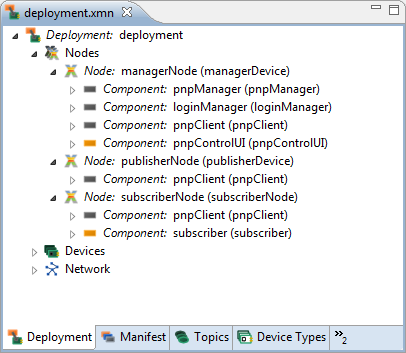
\includegraphics[scale=0.8]{figures/example_configuratorExtension_deployment.png}
	\caption{Deployment model of configurator extension example, showing all three nodes.}
	\label{fig:example_configuratorExtension_deployment}
\end{figure}

The \textit{subscriberNode} contains a single application-defined component of type \textit{subscriber}.
This component simply waits for data on its input port and prints it to the console.
When you navigate to the subscription of this component in its manifest~--~see Figure~\ref{fig:example_configuratorExtension_manifest}~--~%
you can see that it specifies a lower connection bound of $2$ and an upper connection
bound of $3$.

\begin{figure}[htpb]
	\centering
	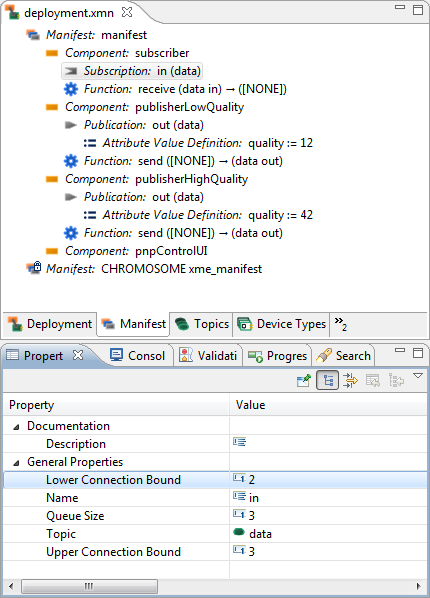
\includegraphics[scale=0.8]{figures/example_configuratorExtension_manifest.png}
	\caption{Manifest of configurator extension example.}
	\label{fig:example_configuratorExtension_manifest}
\end{figure}

The \textit{publisherNode} is initially empty except for the \textit{pnpClient}.
New components will be added to this node at runtime.

The component \textit{pnpControlUI} on the \textit{managerNode} will prompt the user
for plug \& play-related commands. We will use this interface to add new \textit{publisher}s.
There are two kinds of publishers, the \textit{lowQualityPublisher} and the \textit{highQualityPublisher}.
Both publish the same topic but assign different values to the \textit{quality} attribute.
Again you can have a look at these definition in the manifest, see Figure~\ref{fig:example_configuratorExtension_manifest}.

In this example a configurator is registered at the configurator extension.
See Listing~\ref{lst:configuratorExtensionRegistration} for the respective call in the \texttt{managerNode.c} file.
The implementation of the configurator can be found in the following directory:\newline
\texttt{src/configuratorExtension/configurator/demoConfigurator}.
%
The given configurator,
represented by the callback function \lstinline{configuratorExtension_configurator_demoConfigurator_callback()},
will perform the following two tasks:
%
\begin{enumerate}
	\item
		If any input port is connected to less routes than specified in its \textbf{lower connection bound},
		all routes from this port are removed.
		If a new component is to be created that does not satisfy the lower connection bound on one of its ports,
		component creation will be skipped.
	\item
		If any input port is connected to more routes than specified in its \textbf{upper connection bound},
		the excessive routes are removed. Routes with lower quality attribute values are removed first.
		A route with a topic that does not have this attribute is treated as having a quality value of $0$.
\end{enumerate}

\begin{quote}
\textbf{Note:} The removal of already established routes is currently not yet supported,
hence the routes of components that are already created will not be removed.
See Issue \#3952.
\end{quote}

%numbers=left,firstnumber=8842
\begin{lstlisting}[float,label={lst:configuratorExtensionRegistration},caption={Registration of configurator.},breaklines]
// PROTECTED REGION ID(MANAGERNODE_MAIN_RUN_BEFORE) ENABLED START

xme_core_pnp_configExt_addConfigurator
(
    XME_CORE_PNP_CONFIG_EXT_CONFIGURATORTYPE_LOGICAL_ROUTES,
    &configuratorExtension_configurator_demoConfigurator_callback,
    NULL
);

// PROTECTED REGION END
\end{lstlisting}

\noindent To see this behavior in action, run all three nodes and follow these instructions.
You may invoke the \texttt{list nodes} and \texttt{list types} commands to list active nodes and types, respectively.
(the numbers refer to the red numbers in Figure~\ref{fig:example_configuratorExtension_execution}).
\begin{enumerate}
	\item
		The managerNode asks you to enter a command.\newline
		Enter: \texttt{add 2 4100}\newline
		This will add a new component of type \textit{highQualityPublisher} (type ID \texttt{4100}) on the \textit{publisher} node (node ID \texttt{2}).
	\item
		The configurator informs you that the lower connection bound of the subscriber component is not satisfied.
		Therefore it removes the route and the component is not created yet (no output appears on the other nodes).
	\item
		Now enter: \texttt{add 2 4099}\newline
		This will add a new component of type \textit{lowQualityPublisher} (type ID \texttt{4099}) on the publisher node.
	\item
		Now the lower connection bound is satisfied and the new component is plugged.
		After waiting some time you will notice that both publishers start sending.
	\item
		Now enter: \texttt{add 2 4100}
	\item
		An additional \textit{highQualityPublisher} is added and will immediately be plugged in,
		as we now have three routes which is in the limits of the connection bounds of the subscriber.%
		\footnote{Currently having two instances of the same component type will lead to data loss.
		That is why you see a warning on the publisher node after instantiating the second \textit{highQualityPublisher}.
		See also known issue \#3964~\ref{appx:known_issues}.}
	\item
		When you subsequently enter: \texttt{add 2 4100}\newline
		The configurator will inform you that the maximum connection bound is exceeded and
		that it is going to remove the route of the \textit{lowQualityPublisher}.
		As previously noted, established routes cannot be removed yet, so the removal will not actually be executed.
\end{enumerate}

\begin{figure}[htpb]
	\centering
	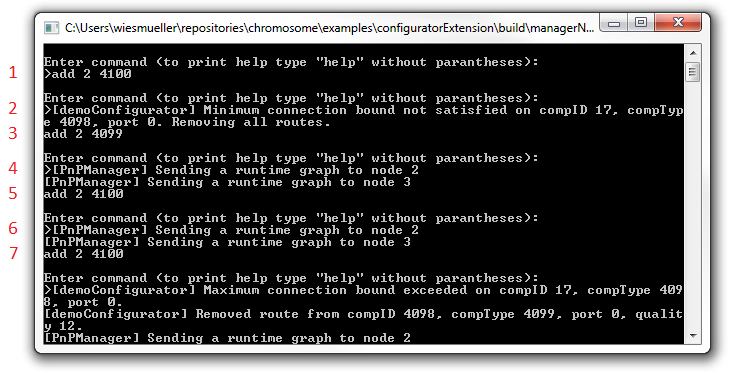
\includegraphics[scale=0.8]{figures/example_configuratorExtension_execution.png}
	\caption{Execution of configurator extension example.}
	\label{fig:example_configuratorExtension_execution}
\end{figure}
